\documentclass[11pt,]{krantz}
\usepackage{lmodern}
\usepackage{amssymb,amsmath}
\usepackage{ifxetex,ifluatex}
\usepackage{fixltx2e} % provides \textsubscript
\ifnum 0\ifxetex 1\fi\ifluatex 1\fi=0 % if pdftex
  \usepackage[T1]{fontenc}
  \usepackage[utf8]{inputenc}
\else % if luatex or xelatex
  \ifxetex
    \usepackage{mathspec}
  \else
    \usepackage{fontspec}
  \fi
  \defaultfontfeatures{Ligatures=TeX,Scale=MatchLowercase}
    \setmainfont[]{Palatino}
    \setmonofont[Mapping=tex-ansi,Scale=0.8]{Source Code Pro}
\fi
% use upquote if available, for straight quotes in verbatim environments
\IfFileExists{upquote.sty}{\usepackage{upquote}}{}
% use microtype if available
\IfFileExists{microtype.sty}{%
\usepackage[]{microtype}
\UseMicrotypeSet[protrusion]{basicmath} % disable protrusion for tt fonts
}{}
\PassOptionsToPackage{hyphens}{url} % url is loaded by hyperref
\usepackage[unicode=true]{hyperref}
\PassOptionsToPackage{usenames,dvipsnames}{color} % color is loaded by hyperref
\hypersetup{
            pdftitle={Learning Options from Data},
            pdfauthor={Pritam Dalal},
            colorlinks=true,
            linkcolor=Maroon,
            citecolor=Blue,
            urlcolor=Blue,
            breaklinks=true}
\urlstyle{same}  % don't use monospace font for urls
\usepackage{natbib}
\bibliographystyle{apalike}
\usepackage{color}
\usepackage{fancyvrb}
\newcommand{\VerbBar}{|}
\newcommand{\VERB}{\Verb[commandchars=\\\{\}]}
\DefineVerbatimEnvironment{Highlighting}{Verbatim}{commandchars=\\\{\}}
% Add ',fontsize=\small' for more characters per line
\usepackage{framed}
\definecolor{shadecolor}{RGB}{248,248,248}
\newenvironment{Shaded}{\begin{snugshade}}{\end{snugshade}}
\newcommand{\KeywordTok}[1]{\textcolor[rgb]{0.13,0.29,0.53}{\textbf{#1}}}
\newcommand{\DataTypeTok}[1]{\textcolor[rgb]{0.13,0.29,0.53}{#1}}
\newcommand{\DecValTok}[1]{\textcolor[rgb]{0.00,0.00,0.81}{#1}}
\newcommand{\BaseNTok}[1]{\textcolor[rgb]{0.00,0.00,0.81}{#1}}
\newcommand{\FloatTok}[1]{\textcolor[rgb]{0.00,0.00,0.81}{#1}}
\newcommand{\ConstantTok}[1]{\textcolor[rgb]{0.00,0.00,0.00}{#1}}
\newcommand{\CharTok}[1]{\textcolor[rgb]{0.31,0.60,0.02}{#1}}
\newcommand{\SpecialCharTok}[1]{\textcolor[rgb]{0.00,0.00,0.00}{#1}}
\newcommand{\StringTok}[1]{\textcolor[rgb]{0.31,0.60,0.02}{#1}}
\newcommand{\VerbatimStringTok}[1]{\textcolor[rgb]{0.31,0.60,0.02}{#1}}
\newcommand{\SpecialStringTok}[1]{\textcolor[rgb]{0.31,0.60,0.02}{#1}}
\newcommand{\ImportTok}[1]{#1}
\newcommand{\CommentTok}[1]{\textcolor[rgb]{0.56,0.35,0.01}{\textit{#1}}}
\newcommand{\DocumentationTok}[1]{\textcolor[rgb]{0.56,0.35,0.01}{\textbf{\textit{#1}}}}
\newcommand{\AnnotationTok}[1]{\textcolor[rgb]{0.56,0.35,0.01}{\textbf{\textit{#1}}}}
\newcommand{\CommentVarTok}[1]{\textcolor[rgb]{0.56,0.35,0.01}{\textbf{\textit{#1}}}}
\newcommand{\OtherTok}[1]{\textcolor[rgb]{0.56,0.35,0.01}{#1}}
\newcommand{\FunctionTok}[1]{\textcolor[rgb]{0.00,0.00,0.00}{#1}}
\newcommand{\VariableTok}[1]{\textcolor[rgb]{0.00,0.00,0.00}{#1}}
\newcommand{\ControlFlowTok}[1]{\textcolor[rgb]{0.13,0.29,0.53}{\textbf{#1}}}
\newcommand{\OperatorTok}[1]{\textcolor[rgb]{0.81,0.36,0.00}{\textbf{#1}}}
\newcommand{\BuiltInTok}[1]{#1}
\newcommand{\ExtensionTok}[1]{#1}
\newcommand{\PreprocessorTok}[1]{\textcolor[rgb]{0.56,0.35,0.01}{\textit{#1}}}
\newcommand{\AttributeTok}[1]{\textcolor[rgb]{0.77,0.63,0.00}{#1}}
\newcommand{\RegionMarkerTok}[1]{#1}
\newcommand{\InformationTok}[1]{\textcolor[rgb]{0.56,0.35,0.01}{\textbf{\textit{#1}}}}
\newcommand{\WarningTok}[1]{\textcolor[rgb]{0.56,0.35,0.01}{\textbf{\textit{#1}}}}
\newcommand{\AlertTok}[1]{\textcolor[rgb]{0.94,0.16,0.16}{#1}}
\newcommand{\ErrorTok}[1]{\textcolor[rgb]{0.64,0.00,0.00}{\textbf{#1}}}
\newcommand{\NormalTok}[1]{#1}
\usepackage{longtable,booktabs}
% Fix footnotes in tables (requires footnote package)
\IfFileExists{footnote.sty}{\usepackage{footnote}\makesavenoteenv{long table}}{}
\usepackage{graphicx,grffile}
\makeatletter
\def\maxwidth{\ifdim\Gin@nat@width>\linewidth\linewidth\else\Gin@nat@width\fi}
\def\maxheight{\ifdim\Gin@nat@height>\textheight\textheight\else\Gin@nat@height\fi}
\makeatother
% Scale images if necessary, so that they will not overflow the page
% margins by default, and it is still possible to overwrite the defaults
% using explicit options in \includegraphics[width, height, ...]{}
\setkeys{Gin}{width=\maxwidth,height=\maxheight,keepaspectratio}
\IfFileExists{parskip.sty}{%
\usepackage{parskip}
}{% else
\setlength{\parindent}{0pt}
\setlength{\parskip}{6pt plus 2pt minus 1pt}
}
\setlength{\emergencystretch}{3em}  % prevent overfull lines
\providecommand{\tightlist}{%
  \setlength{\itemsep}{0pt}\setlength{\parskip}{0pt}}
\setcounter{secnumdepth}{5}
% Redefines (sub)paragraphs to behave more like sections
\ifx\paragraph\undefined\else
\let\oldparagraph\paragraph
\renewcommand{\paragraph}[1]{\oldparagraph{#1}\mbox{}}
\fi
\ifx\subparagraph\undefined\else
\let\oldsubparagraph\subparagraph
\renewcommand{\subparagraph}[1]{\oldsubparagraph{#1}\mbox{}}
\fi

% set default figure placement to htbp
\makeatletter
\def\fps@figure{htbp}
\makeatother

\usepackage{booktabs}
\usepackage{longtable}
\usepackage[bf,singlelinecheck=off]{caption}

\usepackage{framed,color}
\definecolor{shadecolor}{RGB}{248,248,248}

\renewcommand{\textfraction}{0.05}
\renewcommand{\topfraction}{0.8}
\renewcommand{\bottomfraction}{0.8}
\renewcommand{\floatpagefraction}{0.75}

\renewenvironment{quote}{\begin{VF}}{\end{VF}}
\let\oldhref\href
\renewcommand{\href}[2]{#2\footnote{\url{#1}}}

\ifxetex
  \usepackage{letltxmacro}
  \setlength{\XeTeXLinkMargin}{1pt}
  \LetLtxMacro\SavedIncludeGraphics\includegraphics
  \def\includegraphics#1#{% #1 catches optional stuff (star/opt. arg.)
    \IncludeGraphicsAux{#1}%
  }%
  \newcommand*{\IncludeGraphicsAux}[2]{%
    \XeTeXLinkBox{%
      \SavedIncludeGraphics#1{#2}%
    }%
  }%
\fi

\makeatletter
\newenvironment{kframe}{%
\medskip{}
\setlength{\fboxsep}{.8em}
 \def\at@end@of@kframe{}%
 \ifinner\ifhmode%
  \def\at@end@of@kframe{\end{minipage}}%
  \begin{minipage}{\columnwidth}%
 \fi\fi%
 \def\FrameCommand##1{\hskip\@totalleftmargin \hskip-\fboxsep
 \colorbox{shadecolor}{##1}\hskip-\fboxsep
     % There is no \\@totalrightmargin, so:
     \hskip-\linewidth \hskip-\@totalleftmargin \hskip\columnwidth}%
 \MakeFramed {\advance\hsize-\width
   \@totalleftmargin\z@ \linewidth\hsize
   \@setminipage}}%
 {\par\unskip\endMakeFramed%
 \at@end@of@kframe}
\makeatother

\renewenvironment{Shaded}{\begin{kframe}}{\end{kframe}}

\usepackage{makeidx}
\makeindex

\urlstyle{tt}

\usepackage{amsthm}
\makeatletter
\def\thm@space@setup{%
  \thm@preskip=8pt plus 2pt minus 4pt
  \thm@postskip=\thm@preskip
}
\makeatother

\frontmatter

\title{Learning Options from Data}
\author{Pritam Dalal}
\date{}

\begin{document}
\maketitle

\cleardoublepage\newpage\thispagestyle{empty}\null
\cleardoublepage\newpage\thispagestyle{empty}\null
%\cleardoublepage\newpage
\thispagestyle{empty}
\begin{center}
\Large{To Jung Jae-sung (1982 -- 2018),}

\large{a remarkably hard-working badminton player with a remarkably simple playing style}
%\includegraphics{images/dedication.pdf}
\end{center}

\setlength{\abovedisplayskip}{-5pt}
\setlength{\abovedisplayshortskip}{-5pt}

{
\hypersetup{linkcolor=black}
\setcounter{tocdepth}{2}
\tableofcontents
}
\listoftables
\listoffigures
\chapter*{Welcome}\label{welcome}
\addcontentsline{toc}{chapter}{Welcome}

Welcome to the website for \textbf{Learning Options from Data}. This innovative manual will teach you the theoretical and practical fundamentals of options. Like most serious finance books, mathematics will be an invaluable medium for communicating ideas. But unlike standard quantitative treatments of the subject of options, mathematics will not be our only tool. In fact, our primary means of learning and discovery will be the wrangling and analyzing of real-world options data; hence the title: Learning Options from Data.

These pages distill thousands of hours of formal study through the filter of a decade of trading and analysis work in various areas of quantitative finance. I have included only what is useful, timely, and relevant.

This website is \textbf{free to use} and always will be. \textbf{Learning Options from Data} is written in \href{https://rmarkdown.rstudio.com}{RMarkdown} along with \href{https://bookdown.org}{bookdown}. Many thanks to the developers at R Studio for creating such wonderful packages for authoring - this book would not have been possible without those tools.

\chapter{Introduction}\label{introduction}

The purpose of this initial chapter is to provide some context and motivation for how and why I wrote this book. For those of you who want to get to the good stuff, it can safely be skipped.

\section{Delta-Neutral}\label{delta-neutral}

This book would not have been possible without the support of my data partners at \href{http://www.historicaloptiondata.com}{Delta Neutral}. When I was asked to teach a data science course at the University of Minnesota School of Mathematics, I knew I wanted a real-world data set to be the bedrock of the curriculum. A few years prior, I had purchased data from Delta Neutral in order to complete a backtest that I was working on. I was immeasurably impressed with the data, especially when compared to that of their competitors, both in terms of price and quality.

Delta Neutral was founded in 2002 by \href{https://www.linkedin.com/in/rick-fortier-53061a7/}{Rick Fortier}. At the time he was looking for high quality daily option data, and there simply were no reasonable sources. And so he saw a business opportunity. Options data is complex. Rick and his team have hit an unequivocal home run with their product. When I approached Rick about showcasing his data in my courses, he was excited to help spread the knowledge of options and data analysis through this innovative channel.

Nearly all the data analysis examples in this book come from Delta Neutral's Level 3 product. This is a phenomenal data set of the highest quality. It contains daily prices for all options traded on thousands of equity underlyings, and goes back to 2002. Feel free to reach out me, or to the team at Delta Neutral, if you have further questions about their data offerings: \href{mailto:support@deltaneutral.com}{\nolinkurl{support@deltaneutral.com}}.

\section{Why This Book}\label{why-this-book}

This book emanated from a course I was asked to teach for Master of Financial Mathematics (MFM) Program at the University of Minnesota. My initial vision for the course was a short but intensive module on backtesting options trading strategies. It would be geared towards advanced students who had already completed year-long sequences in both options theory and computer programming. The idea was that this module would help the student put their new skills to the test with a challenging data analysis problem - precisely the kind of project they would be required to execute on the job.

Due to a scheduling conflict, this initial vision had to be modified. Instead I would be teaching similar material, but at a more introductory level to the first year students. The typical first year MFM student is a freshly graduated math major with minimal previous exposure to options or programming. So generally very smart students with a solid education, but having little in the way of knowledge that is directly applicable to the task of backtesting options.

As I pondered how I might go about teaching such a course, it occurred to me that I was going to have to present both the basic definition of an option as well as the basic definition of a for-loop. To guide students from that point, to the point of being able to backtest trading strategies struck me as a markedly tall order. But I was intrigued by the challenge and so I accepted.

While designing the course, I knew that I wanted to introduce data analysis material as quickly as possible, but that I was also going to have to cover a lot of options basics up front as well. I quickly realized that basic coding material has been presented exceptionally well in texts such as \href{https://r4ds.had.co.nz/}{R for Data Science}, so I could simply assign readings from these texts as self-study assignments. I also knew that introductory options material has been covered superbly in texts such as Hull and McDonald.

The key motivating insight for me was that many important facts about options can be best illustrated by manipulating options data. As I reflected, I concluded that many of my greatest learning about options came when my hands were very dirty in real-world data (and \emph{NOT} by writing out equations with a pen and a paper). Moreover, by learning about options via programming, you also develop the single most important practical skill for a quantitative finance professional: expressing financial ideas in code.

Thus, I set out to write this new approach finance: \textbf{Learning Options from Data} (LOD).

\section{Who Is This Book For?}\label{who-is-this-book-for}

I classify the target audience for this book in terms of the particular subject matter that they are primarily interested in learning:

\textbf{Options -and- Coding:} The readers who will get the most out of this book will be those that are similar to my MFM students - students who want to learn data analysis in a quantitative finance context, but who still need to build foundations in both areas. My University of Minnesota courses are based on systematically working through this book, as well as completing the \emph{further reading} assignments.

\textbf{Coding:} Suppose you are a professional that has a solid knowledge of options, and you would like to build some additional data analysis skills in R or Python. (Shameless plug: these are precisely the kind of learners that are served by the bespoke training courses from \href{https://pritamdalal.github.io/ods_site/services.html}{Option Data Science}.) You can use this book by jumping straight to the coding exercises, and perusing the explanatory material as needed. You will likely spend a fair amount of time on the prerequisite reading assignments from the coding books mentioned in the next section.

\textbf{Options:} Suppose you are a data scientist or developer that needs to apply their skills in a quantitative finance context. For you, the coding will be simple, but you will need to focus on the explanatory finance material to be able to truly understand the coding assignments. You will spend a fair amount of time on the prerequisite reading assignments from the finance books mentioned in the next section.

\textbf{Delta-Neutral:} If you have already purchased, or are considering purchasing, the Delta-Neutral data set, this book will serve as a guided tour of the data. The coding exercises in this book will greatly accelerate your learning curve. As you probably know, a huge amount time gets spent figuring out a new data set and performing initial wrangling tasks. This book seeks to give you a head start on journey of wrangling the Delta-Neutral data set.

\section{How to Read}\label{how-to-read}

This section details some of the guiding principles I enlisted in writing this book; these provide insights on how to use the book for maximum return on your investment of time.

\subsection{Guiding Philosophies}\label{guiding-philosophies}

\subsubsection*{Coding without Context Sucks}\label{coding-without-context-sucks}
\addcontentsline{toc}{subsubsection}{Coding without Context Sucks}

I have a huge amount of affection for Hadley Wickham's \textbf{R for Data Science} and similar titles. So much so that this book was written in it's image. So much so that this morning I spent 20 minutes figuring how to get my welcome page to look exactly like his.

A general data analysis book like \textbf{R4DS}, by by it's very nature, cannot be context specific. But ultimately, I'm usually left feeling a little bit empty and drowsy performing analysis on toy data sets about cars or flights. The truth is that it's always more enjoyable and effective to learn data analysis when you care about the data. That's really the thrust of this book - learning data analysis in the context of options.

\subsubsection*{Type Along}\label{type-along}
\addcontentsline{toc}{subsubsection}{Type Along}

Pen and paper is dead. If you're not typing code and watching output come out, you're not really learning. The interactive coding environments of R and Python are ideal for this kind of learning. Even if you think you have no idea of what is going on, if there is a coding example, force yourself to type it out (copy/paste doesn't count) and make sure you get the same result.

\subsubsection*{Don't Reinvent the Wheel}\label{dont-reinvent-the-wheel}
\addcontentsline{toc}{subsubsection}{Don't Reinvent the Wheel}

So much for avoiding cliches. The point is that there has been a ton of great introductory material written on both data analysis and options. While I do present my take on some of this material, I also assign reading from a few other texts (which are mentioned below). This book is still only weakly self-contained, and is best studied along side the companion texts.

\subsection{Prerequisites}\label{prerequisites}

The math prerequisite to mastering options is a strong intuitive understanding of calculus, linear algebra, probability, and statistics. For most people, this can really only be acquired from a 3-semester calculus sequence, and semester long undergraduate courses in the other three areas. The options self-help community would probably argue that you don't need that much math, but I disagree. There are certainly diminishing practical returns to advanced subjects like stochastic calculus and functional analysis, but the areas I detail above are a far cry from that.

In my experience, the most productive finance professionals are those who have a strong intuitive understanding of basic undergraduate mathematics, who don't get too caught up in theoretical details, and who focus on implementing their knowledge in code as quickly as possible.

This book is designed for learning data analysis in the context of quantitative finance, but I don't over the basics of either topic (data analysis or quantitative finance) thoroughly. So if you are lacking basic knowledge in either area, you'll need to spend some time on the suggested reading.

\subsection{Further Reading}\label{further-reading}

This book is a hybrid of an introductory data analysis text and an introductory options text. It's a jack of two trades, and master of neither. \textbf{LOD} is designed to be a companion to the books detailed below. Throughout this text, I will assign readings from these other books for one of two reasons: 1) addressing basics that have already been explained well elsewhere; 2) a deeper dive into material for those who want to know more. The amount of further reading you will need will depend on your background and your interests.

\textbf{Data Analysis:}

\emph{R for Data Science} - Hadley Wickham and Garrett Grolemond

\emph{Advanced R} - Hadley Wickham

\emph{Python for Data Analysis} - Wes McKinney

\emph{Python Data Science Handbook} - Jake VanderPlas

\textbf{Quantitative Finance:}

\emph{Options, Futures, and Other Derivatives} - John Hull

\emph{Derivatives Markets} - Robert McDonald

\section{Acknowledgments}\label{acknowledgments}

The layout of this book was adapted from the \texttt{bookdown} files of two great books: \href{https://bookdown.org/yihui/rmarkdown/}{R Markdown: The Definitive Guide} and \href{https://r4ds.had.co.nz/}{R for Data Science}. Thank you to the authors Yihui Xie, J. J. Allaire, Garrett Grolemund, and Hadley Wickham for making the files freely available on Github.

Many thanks to the students at the University of Minnesota, who's questions and curiosities helped to guide the writing of this book.

\section{About the Author}\label{about-the-author}

This book was written by Pritam Dalal, founder of \href{https://pritamdalal.github.io/ods_site/}{Option Data Science} - a boutique consultancy focused on the intersection between data science and volatility markets.

Prior to launching ODS, Pritam held a variety of trading and analysis roles at firms such as Cargill, Wolverine Trading, Allianz Investment Management, and Two Harbors Investment Corp. A common thread running through all of his work has been data-driven analysis, coupled with the ability to communicate those findings to fellow decision makers. These skills have been applied to areas ranging from volatility trading in commodity markets, to equity option market-making, to hedging complex annuities.

In addition to serving clients, Pritam is an adjunct professor in the University of Minnesota School of Mathematics where he \href{https://pritamdalal.github.io/fm5990_site/}{teaches} graduate students about applying data science to quantitative finance.

Pritam holds a Bachelors in Mathematics and Economics from U.C. Berkeley, and a Masters in Financial Mathematics from the University of Minnesota, Twin Cities.

Feel feel to reach him by phone or e-mail: 206.802.5525; \href{mailto:dalal030@umn.edu}{\nolinkurl{dalal030@umn.edu}}.

\chapter{Options 101}\label{options-101}

The purpose of the chapter is to introduce the rudiments of options. We start by building intuition, and introduce formalism as necessary.

Options are simple contracts that show up everywhere in finance. They can be viewed as the building blocks of many other financial instruments. The theory of option pricing serves as the foundation of much of quantitative finance.

Options are insurance contracts wrapped around other financial assets. The asset that is being insured is called the \emph{underlying}. The underlyings we consider in this book are stocks and ETFs, but the essential concepts are the same for other underlyings such as interest rates, corn futures, or barrels of oil.

Let's build some intuition by considering a type of insurance that you are already familiar with: car insurance.

\section{Car Insurance}\label{car-insurance}

Wolverine Trading is a successful market-making firm based in Chicago. The partners at Wolverine would like to get into the car insurance business. They have hired us as consultants to help devise a pricing policy for this new venture.

The type of underlying that Wolverine would like to insure is as follows: a specific driver coupled with a specific vehicle. The driver that is being insured is going to pay Wolverine \emph{premium}. In exchange for the premium, Wolve will reimburse the driver whenever damage to the car exceeds a certain dollar amount, which is called the \emph{strike} of the contract.

\textbf{Intuition Check:} Do you think that Wolverine should charge the same premium irrespective of the underlying? Why or why not?

After some deliberation, we have decided that price differentiation should based on the following contract features and underlying characteristics: strike price, time to expiration, price of the underlying, and volatility of the underlying.

Let's explore these one by one.

\subsubsection*{Price of Underlying}\label{price-of-underlying}
\addcontentsline{toc}{subsubsection}{Price of Underlying}

Sandra is a prospective customer; she has two vehicles that she wants to switch over to Wolve Auto Insurance. One is a busted old Mazda 3 that she bought when she was a struggling graduate student. The other is a fancy self-driving Tesla she bought after starting her lucrative options trading career.

-ADD SIDE BY SIDE PICTURES HERE-

\textbf{Intuition Check:} Which car should be more expensive to insure? Why?

\subsubsection*{Strike Price of Contract}\label{strike-price-of-contract}
\addcontentsline{toc}{subsubsection}{Strike Price of Contract}

Wolverine has three different strike prices that they can offer Sandra for her Tesla:

\begin{itemize}
\tightlist
\item
  \$0 (``at-the-money'')
\item
  \$1,000
\item
  \$5,000
\end{itemize}

\textbf{Exercise:} Order the premium for the three strike prices from cheapest to most expensive. Explain your answers.

\subsubsection*{Time to Expiration}\label{time-to-expiration}
\addcontentsline{toc}{subsubsection}{Time to Expiration}

Wolve Auto has three different contract tenors they can offer to Sandra for her Tesla:

\begin{itemize}
\tightlist
\item
  0.25 years
\item
  0.50 years
\item
  1.00 years
\end{itemize}

\textbf{Exercise:} Order the premium for the three tenors from cheapest to most expensive. Explain your answer.

\subsubsection*{Voltility of Underlying}\label{voltility-of-underlying}
\addcontentsline{toc}{subsubsection}{Voltility of Underlying}

Wolve is pricing insurance for two different customers, Sally and Patty. Both customers are looking to purchase insurance for a fancy new self-driving Tesla. They both want a 1-year contract with with a \$1,000 strike price. Sally's friends describe her as calm, chill, responsible, quiet, serene. On the other hand, Patty's friends describe her: wild, hyper, flaky, loud, and volatile.

\textbf{Intuition Check:} Who should Wolverine charge more for insurance? Why?

\subsubsection*{Insurance Payoff Graph}\label{insurance-payoff-graph}
\addcontentsline{toc}{subsubsection}{Insurance Payoff Graph}

It's 8 a.m. on a Saturday morning. Sally is driving on the freeway heading to her Crossfit class, hands at 10-and-2, eyes intently on the road, soothing classical music playing in the background.

Patty is also driving on the freeway, making her way home from an all night rave. As she drives, she smokes cigarette, touches up her makeup, and then snaps a few selfies for her Instagram story (morning car selfies have the \emph{best} light\ldots{}OMG).

Suddenly, Patty loses control and swerves in front of Sally. Patty is riding dirty and has no insurance. Sally, being her responsible self, made sure to buy a \$1000-strike Wolverine policy as soon as she purchased her vehicle.

Here is a graph of the \emph{payoff} to Sally's insurance contract immediately following the accident. (Make sure to type out this code along with me!!)

\begin{Shaded}
\begin{Highlighting}[]
\NormalTok{strike <-}\StringTok{ }\DecValTok{1000} 
\NormalTok{damage <-}\StringTok{ }\KeywordTok{seq}\NormalTok{(}\DecValTok{0}\NormalTok{, }\DecValTok{3000}\NormalTok{, }\DecValTok{500}\NormalTok{)}
\NormalTok{payoff <-}\StringTok{ }\KeywordTok{pmax}\NormalTok{(damage }\OperatorTok{-}\StringTok{ }\NormalTok{strike, }\DecValTok{0}\NormalTok{)}
\NormalTok{heading <-}\StringTok{ "insurance payoff"}
\KeywordTok{plot}\NormalTok{(damage, payoff, }\DataTypeTok{type =} \StringTok{"n"}\NormalTok{, }\DataTypeTok{main =} \StringTok{"Payoff to Sally"}\NormalTok{)}
\KeywordTok{lines}\NormalTok{(damage, payoff, }\DataTypeTok{type =} \StringTok{"l"}\NormalTok{)}
\end{Highlighting}
\end{Shaded}

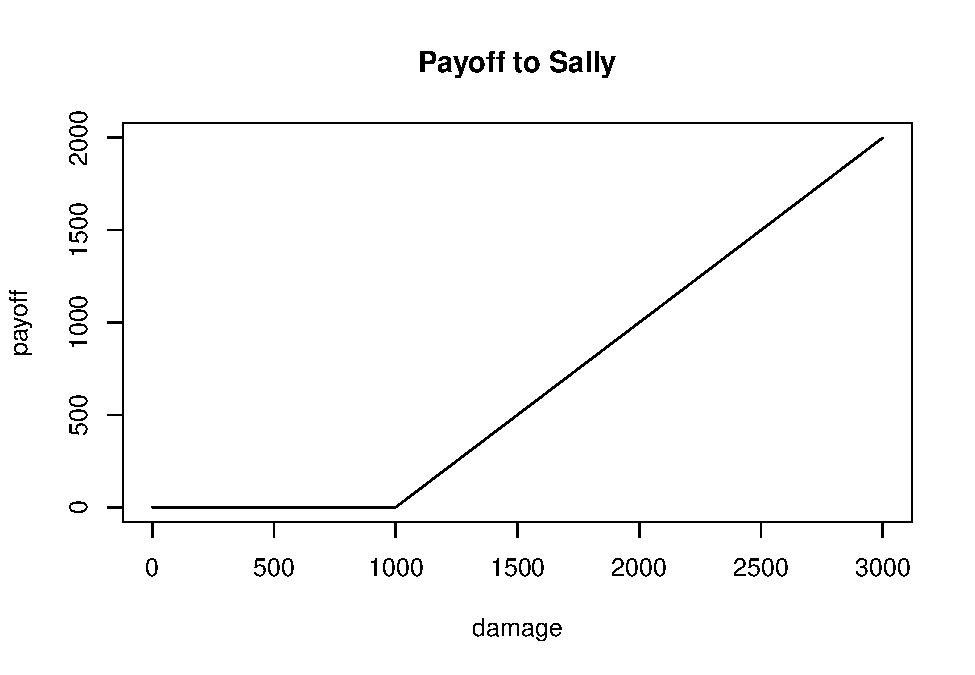
\includegraphics{rmarkdown_files/figure-latex/sally_insurance_payoff-1.pdf}

Notice that if the damage is less than the \$1,000 strike price, Sally receives no reimbursement from her insurance. For every dollar over the strike price, Sally receives a one-for-one payout.

\subsubsection*{Summary}\label{summary}
\addcontentsline{toc}{subsubsection}{Summary}

Let's summarize what we've learned from the previous sections. The following statements are true for car insurance contracts, and also for option contracts:

\begin{enumerate}
\def\labelenumi{\arabic{enumi}.}
\item
  The more valuable the underlying, the more valuable the contract.
\item
  At-the-money strikes are more valuable than out-of-the-money strikes.
\item
  The more time to expiration, the more valuable the contract.
\item
  The more volatile the underlying, the more valuable the contract.
\item
  The payoff function looks like a hockey stick.
\end{enumerate}

\section{Vanilla Options}\label{vanilla-options}

Options come in many different varieties: European, American, Asian, digital, look-back, etc. European and American options are considered the simplest and for that reason they are collectively referred to as \emph{vanilla} options. All other options are considered more complicated and are therefore referred to as \emph{exotic}. Vanilla options are transacted in far greater volumes than exotics, and nearly all publicly traded options are vanilla. In this book we focus exclusively on vanillas.

\subsubsection*{American Options as Insurance}\label{american-options-as-insurance}
\addcontentsline{toc}{subsubsection}{American Options as Insurance}

American (equity) options are insurance contracts that have as their underlying publicly traded stocks. They are called \emph{options} because owning them gives you a \emph{right} to do something, but you are \textbf{not required} to exercise that right. You have the \emph{option} exercise your right if it happens to be beneficial to you. This \emph{right without obiligation} has the effect of creating an insurance benefit for the option holder.

American options come in two varieties: puts and calls. \emph{Put} contracts are insurance for those who already own the underlying stock and intend to sell it in the future; puts are protection against the price of the stock falling before they've had a chance to sell it. \emph{Call} contracts are insurance for those who intend to buy the underlying stock in the future; calls are protection against the price of the stock rising before they've had a chance to buy it.

In reality, you don't have to purchase either puts or calls as insurance. You don't have to own the underlying to buy a put. And if you do happen to own the underlying, you don't have to intend to sell it. Nor do you have to intend to buy the underlying in the future in order to buy calls. You can buy or sell either type of contract to express different views on the underlying.

\subsubsection*{American Option Contract Specification}\label{american-option-contract-specification}
\addcontentsline{toc}{subsubsection}{American Option Contract Specification}

After a lot of intuition building, we are finally ready to give a proper contract specification for American options.

Let's consider American options on some stock \(S\). Calls and puts on \(S\) are defined by two additional contract features: \emph{strike price} and \emph{expiration date}.

\textbf{Call:} a contract that gives the right, but not the obligation, to \textbf{buy} a share of \(S\) at the strike price any time before the expiration date.

\textbf{Put:} a contract that gives the right, but not the obligation, to \textbf{sell} a share of \(S\) at the strike price any time before the expiration date.

\subsubsection*{Option Buyers and Option Sellers}\label{option-buyers-and-option-sellers}
\addcontentsline{toc}{subsubsection}{Option Buyers and Option Sellers}

There are two sides to every options transaction. The \emph{option buyer} pays premium and owns a right. The \emph{option seller}, on the other hand, receives premium and is obligated to respect the right that the buyer has purchased.

In the case of puts, if the option buyer exercises their right to sell the underlying, the option seller is obligated to buy the underlying from them. In the case of calls, if the option buyer exercise their right to buy the underlying, the option seller is obligate to sell the underlying to them.

Sentences like those in the previous paragraph can be a quite confusing at first. There are a lot of ``buys'' and ``sells'' floating around. Don't worry, it will get less confusing over time. But in my experience, you will never outgrown need to occasionally take a deep breath, splash some cold water on your face, and then go back to the contract specifications.

\textbf{Exercises:} Ruobing has purchased an American call on SPY with a strike price of \$250. He paid \$10 in premium. Farez was the option seller on this transaction. It's now the final day of the contract and Ruobing has still not exercised his right.

\begin{enumerate}
\def\labelenumi{\arabic{enumi}.}
\item
  Under what circumstances will Ruobing choose to exercise?
\item
  Under what circumstances does Ruobing make money?
\item
  Under what circumstances does Farez make money?
\item
  What are the min and max of Ruobing's PNL (include premium paid)?
\item
  What are the min and max of Farez's PNL (include premium received)?
\item
  Answer the same questions but for a put with the same strike, expiration, and premium.
\end{enumerate}

\subsubsection*{European vs American}\label{european-vs-american}
\addcontentsline{toc}{subsubsection}{European vs American}

European options are very similar to Americans. The only difference is that the owner of a European option can only exercise their right immediately after the final trading day of the contract. Recall that with Americans, the option holder can \emph{early exercise} at any point before expiration.

To summarize: European options have an exercise date (point). American options have an exercise window - starting today and ending on expiration.

It turns out that in nearly all cases it is not optimal to early exercise an American option (we will explore this in the following chapter). For this reason, we will mostly consider American and European the options as being the same (only the most fastidious quants will take issue with this).

Because there is only one point of time at which a European option can be exercised, the notion of its \emph{payoff function} is straight-forward: it is the value of exercising at the time of expiration. With American options, the notion of a payoff function is complicated by the possibility of early exercise. However, we will lean on the fact that it is almost never optimal to early exercise an American options, and thus define their payoff function as the value of exercising at the time of expiration.

\subsubsection*{Payoff Function}\label{payoff-function}
\addcontentsline{toc}{subsubsection}{Payoff Function}

At this point we will introduce some mathematical notation, as it is the most efficient way to discuss certain aspects of options.

Suppose the current date is \(t\) . Consider a put and call have the same underlying, the same strike price \(K\), and the same expiration \(T\), where \(T > t\). Let \(S_{T}\) be the price of the stock at the time of expiration. We will denote the put buyer's payoff as \(\pi_{b}\), and the call buyer's payoff as \(\pi_{c}\). We can think of these payoffs as functions of \(S_{T}\) and we have that:

Put Buyer Payoff: \(\pi_{p}(S_{T}) = \max \big \{(K - S_{T}),0 \big \}\)

Call Buyer Payoff: \(\pi_{c}(S_{T}) = \max \big \{(S_{T} - K), 0 \big \}\)

\textbf{Exercises:}

\begin{enumerate}
\def\labelenumi{\arabic{enumi}.}
\item
  Convince yourself that the above is true given the contract specification of vanilla puts and call.
\item
  Graph \(\pi_{p}\) and \(\pi_{c}\) as functions of \(S_{T}\).
\item
  Write the expressions for seller's payoff of both puts and calls. Draw the graphs.
\item
  \emph{Total PNL} takes into account the option premium. Let \(m_{p}\) be the put premium and let \(m_{c}\) be the call premium. Modify all four of your graphs to be total pnl functions, rather than payoff functions.
\item
  If we consider \(\pi_{p}\) and \(\pi_{c}\) as functions of \(S_T \in (0, +\infty)\), then both functions are differentiable at all points except for \(S_T = K\).

  \begin{enumerate}
  \def\labelenumii{\alph{enumii}.}
  \tightlist
  \item
    What are the two values of \(\frac{d\pi_{c}}{dS_{T}}\)?
  \item
    What are the two values of \(\frac{d\pi_{p}}{dS_{T}}\)?
  \end{enumerate}
\item
  Recall that the current time is \(t\) and let \(S_{t}\) be the current price of the stock.

  \begin{enumerate}
  \def\labelenumii{\alph{enumii}.}
  \tightlist
  \item
    If you own the put, which inequality do you hope is true between \(S_{t}\) and \(S_{T}\). Which inequality do you hope holds true between between \(S_{T}\) and \(K\)?
  \item
    If you own the call, which inequality do you hope is true between \(S_{t}\) and \(S_{T}\)? How about between \(S_{T}\) and \(K\)?
  \end{enumerate}
\end{enumerate}

\section{Long vs Short}\label{long-vs-short}

If you spend time around financial markets you are likely to encounter the jargon terms and ``short'' and ``long''. These terms can be a bit confusing to the uninitiated, but used in moderation they provide a useful shorthand. In this section we unpack this jargon; we will make use of it throughtout the text.

\subsubsection*{Buyers vs Sellers}\label{buyers-vs-sellers}
\addcontentsline{toc}{subsubsection}{Buyers vs Sellers}

Let's return to the car insurance industry for a moment. In any transaction there is a buyer and a seller. In the car insurance market there are certain classes of entities that buy the insurance, and other classes of entities that sell the insurance. For example, I have purchased policies from State Farm and GEICO. But there would never be a situation in which GEICO or State Farm would buy an insurance policy from me.

Option markets are different in this respect. Various classes of entities - market-makers, hedge-funds, retail traders - buy options as well as sell options. For example, on a given trading day, I may sell an option which a hedge-fund will buy from me on an exchange. On the following day, I may buy a different option from that same hedge fund.

Said in a different way, in the options market, any particular entity can be a buyer of options \emph{and simultaneously} a seller of options.

\subsubsection*{Net Position}\label{net-position}
\addcontentsline{toc}{subsubsection}{Net Position}

As you saw in earlier exercises, the payoff of the option seller is the negative of the payoff of the option buyer. Thus, let us associate the number \(+1\) with the act of buying an option, and associate the number \(-1\) with the act of selling an option contract.

More generally, we can assign a \emph{quantity} number \(Q\) with an options trade. If \(Q > 0\) then the trade is to buy \(Q\) options. If \(Q < 0\) then the trade is to sell \(|Q|\) options.

\textbf{Intuition Check:} What is the payoff function for buying \(Q\) options and holding them until they expire?

Suppose a trader named Lewei has engaged in \(n\) trades on a particular contract \(\mathcal{O}\). And suppose that the quantities of the trades were \(Q_{1}, \ldots, Q_{n}\). Liwei's \emph{net position} in the option \(\mathcal{O}\) is \(Q^{*}\) where

\begin{align*}
Q^{*} = \sum_{i=1}^{n} Q_{i}.
\end{align*}

This concept of net position brings us to our first meanings of \emph{long} and \emph{short}:

\textbf{Long:} If \(Q^{*}>0\) we say that Lewei is \emph{long} \(Q^{*}\) contracts of \(\mathcal{O}\). More generally, we would say that Lewei has a \emph{net long} position in \(\mathcal{O}\).

\textbf{Short:} If \(Q^{*}<0\) we say that Lewei is \emph{short} \(|Q^{*}|\) contracts of \(\mathcal{O}\). More generally, we would say that Lewei has a \emph{net short} position in \(\mathcal{O}\).

Said differently: you are \emph{long} a contract if you are a net buyer of the contract, and we say you are \emph{short} the contract if you are a net seller of the contract.

\subsubsection*{Value}\label{value}
\addcontentsline{toc}{subsubsection}{Value}

The other meaning of long/short has to do with how you fair depending on the direction of change of the price of an asset.

You are said to be \emph{long} an asset if you make money when the value of that asset goes up. You are said to be \emph{short} an asset if you make money when the value of that asset goes down.

So for example, if you hold AAPL in your 401(K), then you are long AAPL because the value of your retirement savings increases when Apple's stock price rises. Similarly, if you have a net short position in a call, then you are short that call (in both senses) because when the value of the call rises, you lose money because that is your liability.

Things get a little confusing when we mix the two meanings of long/short while discussing options. Enjoy the following exercises, such sentences are ubiquitous in options markets. *And remember splash the cold water liberally.)

\textbf{Exercises:}

\begin{enumerate}
\def\labelenumi{\arabic{enumi}.}
\item
  If you have a net long position in a put, are you long or short the underlying?
\item
  If you have a net short position in a put, are you long or short the underlying?
\item
  If you have a net long position in a call, are you long or short the underlying?
\item
  If you have a net short position in a call, are you long or short the underlying?
\end{enumerate}

\chapter{Quantitative Results}\label{quantitative-results}

In this section we consider the basic quantitative foundations of option pricing theory. For a more detailed treatment, I recommend the following execellent texts:

\textbf{Options, Futures, and Other Derivatives} by John C. Hull

\textbf{Derivative Markets} by Robert L. McDonald

\section{Arbitrage}\label{arbitrage}

An \emph{arbitrage} is a risk-less profit that requires no initial investment. One of the basic tenets of quantitative finance is that arbitrage opportunities should not exist in the markets. The reasoning is as follows: if an arbitrage exists, market participants will pile onto the trade and thus move prices until the arb no longer available.

Much of theoretical quantitative finance consists of theorems which are proved by using arbitrage arguements. These theorems often involve questionable assumptions about the market, and they are often of little to use to finance practitioners.

There is, however, a strong kernel of truth in arbitrage arguments. If markets significantly breach so-called \textbf{no arbitrage} prices, then there will be very safe and profitable trades in the market. Traders will eventually catch on to the these trades, which will cause prices to move toward the no-arbitrage levels.

Keep your eyes peeled for arbs in the market. And if you find one, please call me.

\section{Stocks \& Dividends}\label{stocks-dividends}

Companies can raise funds to grow their business by issuing \emph{shares of stock}. The buyer of the stock, called a \emph{shareholder}, pays money to the company which the company keeps forever. In return, the shareholder is entitled to a fraction of the companies future profits and also has the ability to vote on certain matters at shareholder meetings. A crucial point is that the owner of a stock has limited liability with respect to the company. The worst thing that can happen is that shareholder never receives any profits, and the stock itself also becomes worthless. So, for example, if the company is caught illegally polluting, the shareholder cannot be sued for damages. In this sense the value of stock can never be negative.

Once a stock has been issued by a company, the owner of the stock can sell it to another investor. This is called a secondary market transaction. Once the share has been sold in the secondary market, the claims to profits and the voting rights are both transferred to the new owner.

Secondary market transactions occur on exchanges, like the New York Stock Exchange, and are usually what people mean when they talk about \emph{the stock market}. These transactions occur via complicated auction mechanisms that match buyers and sellers. The mechanisms are such that the actual trade prices can fluctuate (sometimes greatly) from one transaction to the next.

Here are some examples of companies who's stocks trade heavily in the secondary markets.

\textbf{AAPL} - Apple

\textbf{GOOG} - Alphabet

\textbf{FB} - Facebook

\textbf{XOM} - Exxon Mobile

Suppose you want to trade a share of stock, and you want to be able to fill your order immediately. If you are a buyer of the stock, you will be charged a certain amount called the \emph{ask} price. If you are a seller of the stock you will receive a certain amount called the \emph{bid} price. The bid price is lower than the ask price. These so-called \emph{bid-ask spreads} exist in other financial markets as well, including options markets.

If you are a market participant for a particular stock, there are at least three different prices that you will need to be aware of. The current bid price, the current ask price, and the last price at which a trade occurred.

Through out the course of this book, we will often refer to \emph{the price of a stock at time} \(t\), and denote it with something like \(S_{t}\). In doing so, we will be referring to one of the following:

\begin{enumerate}
\def\labelenumi{\arabic{enumi}.}
\item
  The current mid price, which is as the average of the bid and ask at time \(t\).
\item
  The last trade price as of time \(t\).
\end{enumerate}

For stocks that have high trading volume, these two values will be usually quite close - but this is not always the case.

For options, which are traded much less frequently than stocks. There is often a much bigger bid-ask spread, and long spans of time between trades, so it is important to clarify what is meant by the phrase \emph{the price at time t}.

The upshot of our previous discussion about exchanges is that \(S_{t}\) varies through time. As it turns out, it is useful to think of the of \(S_{t}\) as a series of random variable. In math circles this is know as a \emph{stochastic process}.

When profits are distributed to the owners of a stock, this is done on a per share basis. The amount that is paid per share is called a \emph{dividend payment}. It is reasonable to wonder whether issuing a dividend payment has any near-term impact on the price of the stock. As it turns out it does, and this question leads to our first \emph{quantitative} result involving an arbitrage argument.

\textbf{Theorem:} Suppose that a stock is going make a divided payment of \(c\) at time \(T\) and that just prior to the dividend payment is trading at a price of \(S^{*}\). Then then price of the stock just after the dividend payment is \(S_{T} = S^{*} - c\).

\textbf{Proof:} NEED TO FILL IN.

Properly defining the concept of a share of \emph{stock} is a complicated legal exercise, and a precise account of how stocks are bought and sold in the secondary market would require its own large book. The amount of detail you will ultimately need know depends on how you intend to apply your knowledge. For example, if you are an attorney that works on IPOs, you will need to know a lot about the legal stuff. If you are a creating statistical arbitrage strategies, you will need be an expert on exchange microstructure.

For the purposes of this book, the following stylized facts will suffice.

\begin{enumerate}
\def\labelenumi{\arabic{enumi}.}
\item
  A shareholder purchases stock which gives them claims to a company's future profits. This is a limited liability investment in that the value of a stock can never be negative.
\item
  After their initial issuance, shares of stock can be bought and sold in the secondary market.
\item
  Trading of stocks on the secondary market occurs on exchanges, with trades occurring thousands or millions of times a day during business hours.
\item
  The exchange creates complex auction mechanisms to match buyers and sellers. The rules of these auctions are such that trades can occur at different prices for every transaction. Trade prices can vary greatly from transaction to transaction.
\item
  The stream of trade prices is often denoted as \(S_{t}\) can be conceptualized as a stochastic process.
\item
  Profits are paid out to shareholders in the form of a per-share payment called a dividend. Immediately after the payment of a dividend, the stock price will reduce by the amount of the dividend.
\end{enumerate}

\section{Exchange Traded Funds (ETFs)}\label{exchange-traded-funds-etfs}

Investing in stocks and other assets is usually an overly costly and complex endeavor for an individual. For this reason, there are various vehicles for small investors to pool their money and for it to be invested as a single fund. The most common form of investment pooling is a \emph{mutual fund}. More esoteric manifestations are hedge funds, unit investment trust (UIT), and real estate investment trusts (REIT). The distinction between these is of general interest, but won't be of huge importance to us in this book.

A fairly recent innovation in the world of pooled investments is exchange traded funds (ETFs). Relative to mutual funds and hedge funds, ETFs engage in simpler strategies that are easier to execute. For this reason, it take fewer people to manage the fund and costs are low. In addition, shares of ETF ownership are traded on exchanges in the exact same way as shares of stock. ETFs pay dividends in the same way that stocks do. Here are some popular ETFs:

\textbf{SPY} - SPDR SP500 - tracks the S\&P500.

\textbf{IWM} - iShares Russell 2000.

\textbf{GLD} - invests in gold futures.

\textbf{XLF} - SPDR Financial - tracks the performance of financial services sector.

In this book we will consider options who's underlyings are stocks and ETFs. We will treat these two underlyings as largely the same.

\section{Discounting \& Accumulating}\label{discounting-accumulating}

When you lend money, you are paid interest to compensate for the fact that you can't use the lent funds for other purposes. In this book we assume that loans are totally safe in that there is no risk of default.

It is useful to conceptualize payment of interest as an \emph{accumulation} over time. We will use the following notation and nomenclature to capture this idea of accumulation:

\textbf{Definition:} Assume the current time is \(t\) and that \(T\) is some time in the future. Then one dollar will accumulate to \(A(t,T)\) by time \(T\). We will call \(A(t,T)\) an \emph{accumulation factor}.

If you are going to receive money in the future, it's not really worth as much to you as if the money were paid right now. The way we account for this value difference is by \emph{discounting} by the amount of interest you could have earned between now when you are going to be paid. This is the notion of \emph{present value}. We express it as follows:

\textbf{Definition:} Let \(t\) be some time before time \(T\). The time \(t\) present value of a one dollar cash flow at time \(T\), will be denoted by \(D(t,T)\). We call \(D(t,T)\) a \emph{discount factor}.

The following statements are true:

\begin{enumerate}
\def\labelenumi{\arabic{enumi}.}
\item
  \(A(t,T) \geq 1\).
\item
  \(D(t, T) \leq 1\).
\item
  \(D(t,T) = A(t,T)^{-1}\).
\end{enumerate}

\textbf{Definition:} Suppose the current time is \(t\). Consider a series of cash flows \(C_{1}, \ldots, C_{n}\) occurring at future times \(t_{1}, \ldots, t_{n}\). Then the time \(t\) present value of this stream of cash flows is defined as:

\begin{align*}
PV(\{ C_{1}, \ldots, C_{n} \}) = \sum_{i = 1}^{n} D(t, t_{i}) \cdot C_{i}.
\end{align*}

\subsubsection*{Forward Accumulating}\label{forward-accumulating}
\addcontentsline{toc}{subsubsection}{Forward Accumulating}

Suppose that the current time is \(t\) and that \(T\) is some time in the (distant) future. Suppose that for all times \(s\) between \(t\) and \(T\), we know the values \(A(t,s)\). This set of accumulation factors is known as the spot yield curve (it is usually quoted as interest rates, but the idea is the same).

Now, suppose for some future time \(t^*\) you want to work out an arrangement with your bank such that you will deposit one dollar at time \(t^*\) and let it accumulate until \(T\). What is the accumulation factor that you should earn? Do you have to wait until time \(t^*\) to find out, or can you lock one in now.

It turns out that this \emph{forward accumulation factor} is determined by the spot yield curve. We will denote the quantity \(A(t, t^*, T)\), and we have that:

\begin{align*}
A(t, T) = A(t, t^*) \cdot A(t, t^*, T)
\end{align*}

\textbf{Proof:}

\section{Option Contracts}\label{option-contracts}

We discussed vanilla (American and European) options at length in the previous chapter. We discuss them here again more formally.

\textbf{NEED TO FINISH}

\section{Forward Contracts}\label{forward-contracts}

Forward contracts are simple derivatives that are one of the foundational building blocks of quantitative finance. The value of forwards are related to option prices via a result known as \emph{put-call parity}, a finding that is seminal to much of derivatives theory.

\subsection{Specification and Payoff}\label{specification-and-payoff}

A forward contract is the obligation to transact some underlying asset at some future date. The transaction occurs at a fixed price, called the \emph{strike price}. The party that agrees to buy the underlying is called the \emph{long} side. The party that agrees to sell the underlying is the \emph{short} side. The underlyings we will consider in this book will be stocks or ETFs, but forwards can exist on any kind of underlying: gold, corn, etc.

The key feature of a forward is that \emph{both} sides are \emph{obligated} to execute their side of the transaction - to either buy our sell the asset, at the agreed upon strike price. This stands in contrast to an option, in which the long side has a right, while the short side has an obligation.

Consider a forward contract struck at \(K\) expiring at time \(T\). Suppose that underlying is trading at \(S_{T}\) at the time of expiration. The long side has agreed to pay \(K\), and in return receives the underlying which has a value of \(S_{T}\). Thus the long position is worth \(S_{T} - K\) at expiration. On the other hand, the short side receives \(K\) but has to deliver the underlying, which is worth \(S_{T}\). So the short position is worth \(K - S_{T}\).

Long Payoff: \(S_{T} - K\)

Short Payoff: \(S_{T} - K\)

\subsection{The Forward Price}\label{the-forward-price}

Suppose that the current time is \(t\) and that we are considering a forward contract that expires at time \(T\). Suppose further that the underlying is currently trading at \(S_{t}\). We are interested in the following question: is there strike price of \(K\) such that both parties can enter into the forward contract for zero cost, without introducing an arbitrage opportunity for either side?

It turns out the answer is yes, an this strike price is of such importance that it has been named simply, \emph{the forward price}. The forward price is determined by two points in time: the current time \(t\) and the expiration time \(T\). We will denote the forward price associated with these two times as \(F(t, T)\).

\textbf{Forward Pricing Formula:} Suppose we are considering a forward contract at time \(t\) which expires at time \(T\). Suppose that the underlying is currently trading at \(S_{t}\) and that during the life of the forward, the underlying stock pays dividends \(c_{1}, \ldots, c_{n}\) at times \(t_{1}, \ldots, t_{n}\). Then the we have that:

\begin{align*}
F(t, T) &= A(t, T) \cdot S_{t} - \sum_{i=1}^{n} A(t, t_{i}, T) \cdot c_{i}
\end{align*}

\textbf{Proof:}

In words, we have that the forward price is the accumulated value of the current stock price less the accumulated value of all the dividend payments during the life of the contract.

Notice that for non-dividend paying stocks, the forward price is simply the accumulated value of the current stock price: \(F(t, T) = A(t, T) \cdot S_{t}\).

\subsection{Valuing a Forward Contract}\label{valuing-a-forward-contract}

Suppose that you enter into a forward contract at time \(t^{*}\) and the strike price \(K\) was chosen such that both parties could enter into the contract for zero cost. Suppose that the time is now \(t > t^{*}\), what would be the value to unwind this contract?

\textbf{Fact:} The no arbitrage unwind value of this contract is \(D(t, T) \cdot (F(t, T) - K)\).

\textbf{Proof:}

This result really has nothing to do with the fact that the forward contract entered into at time \(t^{*}\) or that it's initial strike what chosen to make it a zero value contract. Ultimately it just gives us a formula for valuing a forward contract at any point.

Notice that if a forward contract is struck at the current forward price, then it has zero value, which we would expect.

\subsection{Synthetic Forwards}\label{synthetic-forwards}

A portfolio consisting of a long call and a short put is a synthetic forward position. More specifically, you simultaneously hold a long call and a short put, both with the same strike \(K\), and both expiring at the same time \(T\), then your payoff at time \(T\) will be the same as a long forward contract struck at \(K\) and expiring at \(T\). Let's see how this is the case.

Let the current time be \(t\). Consider a call and put on the same underlying, with the same strike price \(K\), that both expire at time \(T\). If you have a long position in the call and a short position in the put, then in all states of the world at time \(T\) this portfolio has a value of \(S_{T} - K\), which is the same value as the payoff as a long forward.

Suppose that \(S_{T} > K\). You exercise your long call, for which you receive the stock worth \(S_{T}\) while paying the strike price \(K\) for it. The put you are short expires worthless. The total value of these two positions is \(S_{T} - K\).

On the other hand, suppose \(S_{T} < K\). Your short put position will be exercised, forcing you to buy the stock for \(K\) even though it is only worth \(S_{T}\). Your call is worthless, so you won't exercise. Once again, the combined value of these two position is \(S_{T} - K\).

If \(S_{T} = K\), nothing happens because both options are worthless. Doing nothing has zero value. But of course in this situation we have that \(S_{T} - K = 0\).

\section{Put-Call Parity}\label{put-call-parity}

Our discussion of synthetic forwards leads us to one of the most important results in all of derivatives theory: \emph{put-call parity}.

Let the current time be \(t\). Consider a put and a call that both expire at time \(T\), both struck at \(K\). We know that the long call combined with the short put create a synthetic forward with strike price \(K\). From previous sections we also know how to value a forward contract. Putting these two results together we get following put-call parity identity:

\begin{align*}
C(t, T, K) - P(t, T, K) = D(t, T) \cdot (F(t, T) - K).
\end{align*}

Let's examine a couple special cases more closely.

\subsubsection*{Non-Dividend Paying Stock}\label{non-dividend-paying-stock}
\addcontentsline{toc}{subsubsection}{Non-Dividend Paying Stock}

Recall that when the stock pays no dividends during the life of the forward, that the forward price is simply the accumulated spot price. Thus, we have

\begin{align*}
C(t, T, K) - P(t, T, K) &= D(t, T) \cdot (F(t, T) - K) \\
                        &= D(t, T) \cdot (A(t, T) \cdot S_{t} - K) \\
                        &= S_{t} - D(t, T) \cdot K.
\end{align*}

\subsubsection*{Dividend Paying Stock}\label{dividend-paying-stock}
\addcontentsline{toc}{subsubsection}{Dividend Paying Stock}

Suppose that during the life of the options the underlying stock pays dividends of \(c_{1}, \ldots, c_{n}\) at times \(t_{1}, \ldots, t_{n}\). Then we have that

\begin{align*}
C(t, T, K) - P(t, T, K) &= D(t, T) \cdot (F(t, T) - K) \\
                        &= D(t, T) \cdot \bigg(A(t, T) \cdot S_{t} - \sum_{i=1}^{n} A(t, t_{i}, T) \cdot c_{i} - K \bigg) \\
                        &= S_{t} - PV(\{c_{1}, \ldots, c_{n} \}) - D(t, T) \cdot K.
\end{align*}

\section{Rational Option Pricing}\label{rational-option-pricing}

The Black-Scholes pricing framework, which we will discuss at length in later chapters, requires complex assumptions about the random nature of the underlying, and dynamic trading strategies for replicating option payoffs. These complexities are required to give a specific value of to an option. But there is a actually a lot we can say about option prices without making any assumptions of the underlying. This line of reasoning is called \emph{rational option pricing}.

Not only does rational pricing yield practically useful results, understanding these arguments helps to build intuition about options.

\subsubsection*{Extreme American Bounds}\label{extreme-american-bounds}
\addcontentsline{toc}{subsubsection}{Extreme American Bounds}

Our first results place crude bounds on the price of options.

The worst thing that can happen with either a long put or long call position, is that it is not exercised. So vanilla options can never have negative value.

As a call buyer, the best outcome is that you exercise, which results in owning the stock Thus, call can never be worth more than the underlying stock. As a put buyer, the best outcome is that you exercise when the stock is worthless, and you receive \(K\). Thus, the put can never be worth more that \(K\).

These facts are summarized in the following inequalities:

\begin{align*}
0 &\leq C_A(S, K, T) \leq S \\
0 &\leq P_A(S, K, T) \leq K.
\end{align*}

\subsubsection*{\texorpdfstring{Americans \(\geq\) European}{Americans \textbackslash{}geq European}}\label{americans-geq-european}
\addcontentsline{toc}{subsubsection}{Americans \(\geq\) European}

Any strategy that you can execute with a European option, you can execute with the American variant as well. Thus, American are worth at least as much as their European equivalents. This is summarize with the following inequalities:

\begin{align*}
C_E(S, K, T) &\geq C_A(S, K, T) \\
P_E(S, K, T) &\geq C_A(S, K, T).
\end{align*}

\subsubsection*{Call Bounds}\label{call-bounds}
\addcontentsline{toc}{subsubsection}{Call Bounds}

We can string together put-call parity along with the previous two results (add equation numbers), to arrive at the following series of inequalities:

\begin{align*}
\text{max}\big\{ 0, D(t, T) \cdot ((F(t, T) - K))  \big\} \leq C_E(S, K, T) \leq C_A(S, K, T) \leq S.   
\end{align*}

From left to right, the justification for these three are as follows:

\begin{enumerate}
\def\labelenumi{\arabic{enumi}.}
\item
  Extreme lower bound combined with put-call parity. Notice that this is equivalent to saying that a vanilla call is always worth more than it's intrinsic value.
\item
  Americans are worth more than Europeans.
\item
  Extreme upper bound for Americans.
\end{enumerate}

\subsubsection*{Put Bounds}\label{put-bounds}
\addcontentsline{toc}{subsubsection}{Put Bounds}

We can argue for a similar sequence of inequalities for puts:

\begin{align*}
\text{max}\big\{ 0, D(t, T) \cdot (K - F(t, T))  \big\} \leq P_E(S, K, T) \leq P_A(S, K, T) \leq K. 
\end{align*}

Here is the justification:

\begin{enumerate}
\def\labelenumi{\arabic{enumi}.}
\item
  Extreme lower bound combined with put-call parity. Notice that this is equivalent to saying that a vanilla put is always worth more than intrinic.
\item
  Americans are worth more than Europeans.
\item
  Extreme upper bound for Americans.
\end{enumerate}

\subsubsection*{Early Exercise No Dividends}\label{early-exercise-no-dividends}
\addcontentsline{toc}{subsubsection}{Early Exercise No Dividends}

It is never optimal to early exercise an American call option on a non-dividend paying stock. For a non-dividend paying underlying, it is always better to sell the call than to exercise. To see this, recall that from put call parity we have that

\begin{align*}
C_E(S_t, K T) &= D(t, T) \cdot (F(t, T) - K) + P_E(K, T) \\
            &= D(t, T) \cdot (A(t, T) \cdot S_t - K)) + P_E(S_t, K, T) \\
            &= S_t - D(t, T) \cdot K + P_E(S_t, K, T).
\end{align*}

If we can show that \(S_t - D(t, T) \cdot K + P_E(K, T) > S_t - K\) then we are done, because American options are always worth at least as much as Europeans. This inequality is equivalent to

\begin{align*}
K > D(t, T) \cdot K - P_E(S_t, K, T) \iff \\
K\cdot(1 - D(t, T)) + P_E(S_t, K, T) > 0
\end{align*}

But of course this final inequality is true because \(D(t, T) < 1\) and \(P_E(S_t, K, T) > 0\).

\subsubsection*{Early Exercise Single Dividend}\label{early-exercise-single-dividend}
\addcontentsline{toc}{subsubsection}{Early Exercise Single Dividend}

(NOT COMPLETE) Consider and American call on a stock that pays a single dividend, call it \(\delta\), before the option expires, say at time \(t^*\). From put-call parity we have

\begin{align*}
C_E(S_t, K, T)  &= D(t, T) \cdot (F(t, T) - K) + P_E(S_t, K, T) \\
                &= D(t, T) \cdot (A(t, T) \cdot S_t - D(t, t^*)\delta - K) + P(S_t, K, t) \\
                &= S_t - D(t, T) \cdot D(t, t^*) \delta - K \cdot D(t, T) + P(S_t, K, t)
\end{align*}

\chapter{The Markets}\label{the-markets}

In order to participate in options markets you need to have a basic understanding of how they work.

\section{Exchanges}\label{exchanges}

\section{Brokers}\label{brokers}

\section{Market-Makers}\label{market-makers}

\section{Other Liquidity Providers}\label{other-liquidity-providers}

\section{The Buy Side}\label{the-buy-side}

\chapter{Profit \& Loss}\label{profit-loss}

The most basic and important performance measure of a trading strategy is its daily \emph{profit and loss}, which we usually shorten to simply \emph{PNL}. In subsequent chapters, we will encounter a variety of theoretical statements regarding the pricing and hedging of options; many of these can be easily translated into statements about PNL. It is my opinion that analyzing PNLs is the best way to internalize knowledge of options, which is in part why I wrote this book.

In this chapter we consider how to calculate profit and loss for stocks and options trades.

\section{Stock PNL}\label{stock-pnl}

As mentioned above, once fractional limited liability ownership of companies has been created via the initial issuance of stocks, that stock can be traded in the secondary market. These trades occur on exchanges, all throughout the trading day, and most of the stocks that you are familiar with (GOOG, AAPL, FB) trade tens of thousands of times a day, with millions of shares being transacted on a daily basis.

At the end of each trading day, it is a market convention to take note of where a particular stock was trading just before the close of the market. This price is often referred as the settle price for that day. They exact way that settlement prices are determined is outside the scope of this book.

Daily settle prices will be relevant to us for two reasons:

\begin{enumerate}
\def\labelenumi{\arabic{enumi}.}
\item
  Settle prices are used to determine the payoff of an option.
\item
  Settle prices are used to determine the daily PNL of a stock position.
\end{enumerate}

In this section we will concern ourselves with \#2.

As a matter convention, we will let natural numbers, indexed with \(i\), represent consecutive trading days. And we will let \(S_{i}\) prepresent the price of a particular stock on day \(i\).

\subsection{Marking to Mid}\label{marking-to-mid}

Let \(\mathcal{S}\) be a particular stock. Suppose we purchase one share of it in the middle of the day 1, and that the trade price is \(S^{*}\). Now, let \(S_{i}\) be the settle price for day \(i=1,\ldots,n\).

We seek to define the following:

\textbf{Daily:} \(D_{i}\) - the \emph{daily PNL} for the trade as of end-of-day \(t_i\).

\textbf{TTD:} \(C_{i}\) - the \emph{trade-to-date PNL} for the trade as of end-of-day \(t_i\).

\begin{align*}
D_{i} &= \begin{cases} S_{1} - S^{*} & i = 1 \\ S_{i} - S_{i-1} & i > 1 \end{cases} \\[10pt]
C_{i} &= \sum_{k=1}^{i} D_{k} = S_{i} - S^{*}
\end{align*}

The fact that \(C_{i} = S_{i} - S^{*}\) can be interpreted with the following intuitive statement: the stock purchase is worth the difference between its current price, and what you paid for it.

This is a simple calcluation that is perfectly fine in many situation. The tacit assumption is that if you unwound your position, you would do so at the mid prices. However, this isn't quite true in practice, and depending on your application, and the availability of the data, you may want to incorporate the fact that you would have to unwind at the bid. This is what we will do in the next section.

\subsection{Marking to Bid}\label{marking-to-bid}

Suppose now that instead of a single end of day mid price, we have two end of day prices: a bid price and ask price, denoted \(B_{i}\) and \(A_{i}\). In this situation, \(S_{i}\) would lie between

If we are marking our stock trade to the bid, the we would need to modify the definiton of our daily and cumulative PNL as follows:

\begin{align*}
D_{i} &= \begin{cases} B_{1} - S^{*} & i = 1 \\ B_{i} - B_{i-1} & i > 1 \end{cases} \\[10pt]
C_{i} &= \sum_{k=1}^{i} D_{k} = B_{i} - S^{*}
\end{align*}

By marking to the bid, we are accounting for the fact that if we were to exit our long stock position, we would sell the stock, and we would have to sell the stock at the bid. If you are analyzing a trading system the involves frequent opening and closing of positions, then it is important to account for bids and asks in your PNL calcuations.

\section{Option PNL}\label{option-pnl}

Suppose we trade an option \(\mathcal{O}\) at a price \(P\) on trade date \(t_{1}\), and we hold that position until expiration, which is trade date \(t_{n}\). The letter \(i\) will serve as an index over the trade dates, so \(i = 1,\ldots,n\).

Let \(B_{i}\) and \(A_{i}\) be the end-of-day bid and ask prices of the option for trade date \(t_{i}\). Note that both \(B_{n}\) and \(A_{n}\) are equal to the option payoff. We seek to define the following:

\textbf{Daily:} \(D_{i}\) - the \emph{daily PNL} for the trade as of end-of-day \(t_i\).

\textbf{TTD:} \(C_{i}\) - the \emph{trade-to-date PNL} for the trade as of end-of-day \(t_i\).

Intuitively, the trade-to-date (TTD) PNL is the amount of money you made or lost if you unwind the trade at current market values. The daily PNL is the one day change in the trade-to-date PNL. The two concepts are interchangeable in that it is possible to define TTD PNL in terms of daily PNL, and vice versa.

In my own work, I prefer to calculate daily PNLs for a trade, and then define the trade-to-date PNL as the sum of the previous daily PNLs. We will consider both alternatives below. It is useful to consider buys and sells separately.

\subsection{Total PNL At Expiration}\label{total-pnl-at-expiration}

The easiest PNL concept for an option trade is the the total PNL at the time of expiration.

Suppose option \(\mathcal{O}\) at a price \(P\) on trade date \(t_{1}\), and we hold that position until expiration, which is trade date \(t_{n}\). Let \(\Pi\) be the payoff of the option. Then at the time of expiration, the total PNLs for for the long and shorts positions2 are as follows:

Long: \(\Pi - P\)

Short: \(P - \Pi\)

\subsubsection*{TTD as Sum of Daily - Buy}\label{ttd-as-sum-of-daily---buy}
\addcontentsline{toc}{subsubsection}{TTD as Sum of Daily - Buy}

\begin{align*}
D_{i} &= \begin{cases} B_{1} - P & i = 1 \\ B_{i} - B_{i-1} & i > 1 \end{cases} \\[10pt]
C_{i} &= \sum_{k=1}^{i} D_{k}
\end{align*}

~

\textbf{Exercise:} Show that \(C_{j} = B_{j} - P\).

\subsubsection*{TTD as Sum of Daily - Sell}\label{ttd-as-sum-of-daily---sell}
\addcontentsline{toc}{subsubsection}{TTD as Sum of Daily - Sell}

\begin{align*}
D_{i} &= \begin{cases} P - A_{1} & i = 1 \\ A_{i-1} - A_{i} & i > 1 \end{cases} \\[10pt]
C_{i} &= \sum_{k=1}^{i} D_{k}
\end{align*}

~

\textbf{Exercise:} Show that \(C_{i} = P - A_{i}\).

\subsubsection*{Daily as Change in TTD - Buy}\label{daily-as-change-in-ttd---buy}
\addcontentsline{toc}{subsubsection}{Daily as Change in TTD - Buy}

\begin{align*}
C_{i} &= B_{i} - P \\[10pt]
D_{i} &= \begin{cases} C_{1} & i = 1 \\ C_{i} - C_{i-1} & i > 1 \end{cases}
\end{align*}

~

\textbf{Exercise:} Show that both formulations of \(D_{i}\) are equivalent.

\subsubsection*{Daily as Change in TTD - Sell}\label{daily-as-change-in-ttd---sell}
\addcontentsline{toc}{subsubsection}{Daily as Change in TTD - Sell}

\begin{align*}
C_{i} &= P - A_{i} \\[10pt]
D_{i} &= \begin{cases} C_{1} & i = 1 \\ C_{i} - C_{i-1} & i > 1 \end{cases}
\end{align*}

~

\textbf{Exercise:} Show that both formulations of \(D_{i}\) are equivalent.

\section{Scaling Up}\label{scaling-up}

In a professional setting, it is rare that you will calculate the PNL of a single stock trade or options trade. Rather, you will want to calculate the PNL of a portfolio of trades. Conceptually this is quite simple, as the daily PNL of a collection of trades is simply the sum of the daily PNL of the individual trades. In practice, for large numbers of trades, you have to be careful because unforseen errors - say from missing data, or an erroneous price - can be hard to identify.

{[}CODING EXERCISE{]}

\section{Returns}\label{returns}

While PNL is an important performance metric, it is often hard to interpret without first normalizing by the amount of capital required to fund the investment. This is precisely what the notion of a return is.

\chapter{Option Pricing}\label{option-pricing}

What \emph{should} the price of an option be at any given point in time? This seems like an innocent question, but it took the collective quantitative finance community over one hundred years to answer in a satisfactory way. Along the way modern finance was born.

\section{Black-Scholes-Merton}\label{black-scholes-merton}

In the 1970s, decades of option pricing research coalesced into a pricing framework that yielded a fairly simple formula for pricing vanilla options. It is known as the Black-Scholes framework, being named after two of major contributers to it's development Understanding the framework is more important than memorizing the formula.

The upshot of the BSM pricing framework is that given several contract features, and several market values, you can assign a value to an option.

\textbf{Contract Features}

\begin{itemize}
\item
  p/c - put or call
\item
  \(K\) - strike price
\item
  T - expiration date (time to expiration)
\end{itemize}

\textbf{Market Values}

\begin{itemize}
\item
  \(S_{t}\) - current underlying price
\item
  \(\sigma\) - estimate of the standard deviation log-return of the price of underlying between now and expiration
\item
  \(\delta\) - estimate of dividends paid over the life of the option
\item
  \(r\) - risk-free interest rate
\end{itemize}

All the inputs of the BSM formula are readily observable, except for \(\sigma\), also called volatility. The options market is the \emph{volatility} markets. The market for the underlying stock is the \emph{expected-return} market.

\textbf{Question:} Suppose Jake is an SPY trader for Wolverine and that on a given day, the price of SPY drops by 10\%. Should Jake increase or decrease \(\sigma\) in his pricing models?

\section{Investment Risk Reduction}\label{investment-risk-reduction}

The ultimate goal of this section is to discuss delta-hedging and option replication. However, the notion of hedging in an derivatives context is often confused with two other ideas in finance, so I want to spend some time teasing them apart. Towards this end we will discuss three related concepts: - diversification of investments - hedging of investments - hedging for derivatives replication (including delta-hedging) \vspace{10pt}

These three are related in that they are all manifestations of risk reduction.

\subsubsection*{Diversification of Investments}\label{diversification-of-investments}
\addcontentsline{toc}{subsubsection}{Diversification of Investments}

Let \(X_1\), \(X_2\) be two random variables with the same variance and \(corr(X_1, X_2) < 1\). Then we have that

\begin{align*}
sd(0.5 \cdot X_1 + 0.5 \cdot X_2) < sd(X_1) = sd(X_2).
\end{align*}

The financial intuition of this result is: if you are investing, and you have a choice between two assets that are equally risky (i.e.~the same variance of returns), then you will always lower the riskiness of your portfolio by \emph{diversifying} over both assets, rather than just investing in one. This result can be generalized to \(n\) random variables.

Spread your money over many different non-perfectly correlated investments and you will reduce your overall portfolio risk.

\textbf{Exercises:}

\begin{enumerate}
\def\labelenumi{\arabic{enumi}.}
\item
  Use the \texttt{tidyqant} package to download 5 years of SPY and IWM price data from Yahoo finance.
\item
  Use the adjusted close prices to calculated daily log-returns for each ETF.
\item
  Calculate the standard deviation of the daily returns for both, and then create a seriese of scaled prices for IWM so that the scaled prices has the same standard deviation as SPY.
\end{enumerate}

\subsubsection*{Hedging of Investments}\label{hedging-of-investments}
\addcontentsline{toc}{subsubsection}{Hedging of Investments}

Hedging in an investment context can be thought of as an extreme form of diversification. Suppose you have a position in some asset \(A\). Suppose you believe that asset \(B\) has a strong anti-correlation with \(A\): when the price of \(A\) goes down, the price of \(B\) goes up, and vice-versa. If you were to invest in asset \(B\) for this reason, it would be referred to as a \emph{hedge against} \(A\).

In investments, diversification (previous concept) exploits uncorrelatedness, while hedging exploits anti-correlation.

\textbf{Exercises:}

\begin{enumerate}
\def\labelenumi{\arabic{enumi}.}
\item
  Use the \texttt{tidyquant} package to download 5 years of SPY and GDX price data from Yahoo finance.
\item
  Google the GDX ETF and find out what it's all about.
\item
  Suppose at the beginning of the 5 year period that you have \$125K to invest.
\item
  You know that for sure you are going to invest \$100K in SPY, but you're not sure what to do with the additional \$25K.
\item
  You consider two options:

  \begin{itemize}
  \tightlist
  \item
    keep it in cash
  \item
    invest in GDX
  \end{itemize}
\item
  Compare the standard deviation of the portfolio returns for each choice.
\item
  GDX is negatively correlated with SPY, so it would be a hedge in the investment sense. Confirm this by comparing the standard deviations of the two portfolios and also by visualizing with \texttt{ggplot()}.
\end{enumerate}

\section{Forward Replication}\label{forward-replication}

Hedging in the context of derivatives means something quite different. It refers to engaging in a set of trades - called a \emph{replicating portfolio} - that perfectly replicates the payoff of a derivative. If you can find such a replicating portfolio, and that replicating portfolio has a a known cost, then that is the \emph{no arbitrage} price of the derivative.

Hedging is a both a theoretical pricing technique, and also a prescription for action for a trading desk that deals derivative contracts to its customers.

Yuchen works for Wolverine Trading's forward contract desk. Yifei is one of Yuchen's customers and would like to engage in a forward contract to buy a single share of SPY, 2 months from now.

Suppoe th the current price of SPY is 265, and that the two-month interest rate is 1\%. Suppose further that SPY does not pay any dividends between now and the expiration date of the forward contract. The price which Yifei agrees to buy SPY in 2 months is called the strike price. Let's call it \(K\).

If \(K = 265 \cdot (1 + 0.01) = 267.65\), the forward contract has zero cost at the time of inception. The reason for this is that Yuchen can create a replicating portfolio for zero cost right now, that perfectly matches the payoff/obligations of the derivative. Yuchen's replicating portfolio consists of the following: - he borrows 265 for two months (short a bond) - he buys a share of SPY (long the underlying)

When the contract expires, Yuchen will collect 267.65 from Yefei and deliver the the stock. With the 267.65 that Yuchen collected, he will repay his loan, the balance of which is exactly 267.65.

If Yuchen were to charge a slightly higher forward price on his contract, say 270, then engaging in the foward contract would yield 3.35 in riskless profit, two months from the inception of the contract, which at that time has a present value of \(3.35 \cdot (1 + 0.01)^{-1} = 3.32\). Notice that Yuchen takes no risk, which is the ideal situation for a derivatives desk.

This replicating portfolio does two thing for us: - gives us a way to argue zero cost forward price - gives Yuchen a prescription for action in his derivatives business

Yuchen's trades - selling a bond and buying underlying - are collectively an example of a \emph{static hedge}. The portfolio is static in that doesn't require any adjustments during the life of the contract - Yuchen can set it and forget it.

More complicated derivatives, like vanilla options, require \emph{dynamic hedging}.Their replicating portfolios which must be adjusted frequently.

\section{Delta Hedging}\label{delta-hedging}

The BSM framework is a means for determining the price of an option, call it \(P\). It makes some stylized assumptions about the nature of the underlying and the market for the underlying: - thee underlying price process \(S_{t}\) follows a geometric brownian motion - markets trade continuously without a bid-ask spread

The BSM posits that to hedge/replicate an options position, that we simply need to hold \(-\frac{\partial P}{\partial S_{t}}\) units of the underlying at any point in time. Holding \(-\frac{\partial P}{\partial S_{t}}\) units of the underlying is referred to as \emph{delta-hedging}. Notice that \(\frac{\partial P}{\partial S_{t}}\) is a constantly changing quantity, so you have to rebalance our delta-hedge frequently, which is what makes this a \emph{dynamic} hedging strategy.

The BSM assumptions are demostrably false, but they are close enough to being right that delta-hedging is a useful practice for derivatives dealers and options market-makers.

As mentioned above, BSM assumes that \(S_{t}\) follows a geometric brownian motion. The is equivalent to saying that log-return of \(S_{t}\) over any time scale is normally distrubuted, and that returns over disjoint time periods are independent: wrong and wronger.

For the purposes the option pricing, the most important feature of the GBM price process \(S_{t}\) is it's volatility, which is typically denoted \(\sigma\). Volatility is the standard-devation of the log-returns over one unit of time (the industry standard is to quote \(\sigma\) for one year).

Great news: Yuchen has been promoted to Wolverine's option's desk and his best customer Yefei has upgraded from forwards to buying call options on SPY. Let's suppos that Yuchen and Yefei live in a Black-Scholes world.

Yefie is in the market for a call option, and reaches out to Yuchen to try to get a deal done. Yuchen predicts that the volatility of SPY will be \(\sigma_{*}\) over the life of the option, for which BSM gives a price of \(P_{*}\).

Yuchen sells Yefei the call option - charging \(P_{*}\) - and then engages in dynamic delta-hedging. He rebalances his delta daily.

Suppose that the realized volatilty of SPY during the life of the option is \(\sigma_{r}\) and that the BSM price for that volatility would have been \(P_{r}\). They Yuchen's PNL will be \emph{approximately}:

\begin{align*}
P_{*} - P_{r} = V * (\sigma_{*} - \sigma_{r})   
\end{align*}

where \(V\) is the vega of the option. This is PNL is approximate because of discrete daily delta-hedging. If Yuchen delta-hedged continuously, as BSM prescribes, this PNL would be exact and deterministic.

Notice that Yuchen's PNL is a function of the difference between his pricing volaililty (implied) and the realized volatility. One of the major insights of the BSM framework is that a delta-hedged option position is a position in realized volatility. Intuition: an option price function has positive curvature (gamma). By delta hedging, you are removing the linear part of the option price changes, but there are still the second-order effects of changes in the price of the underlying.

If you have a short delta-hedged option position, then your delta-hedging will often have you buying high and selling low. Not good.

\textbf{Facts about Delta-Hedged Options Positions:}

\begin{enumerate}
\def\labelenumi{\arabic{enumi}.}
\item
  Consider a call and put with the same underlying, strike, and expiration. Then the delta-hedged call is equivalent to the delta-hedged put.
\item
  The PNL of a naked option position will have a higher variance than the PNL of it's delta-hedged counterpart. But the PNL variance of the delta-hedged position is not zero.
\item
  A long delta-hedged option position is long realized volatility.
\item
  A short delta-hedged option position is short realized volatility.
\end{enumerate}

\section{Greeks}\label{greeks}

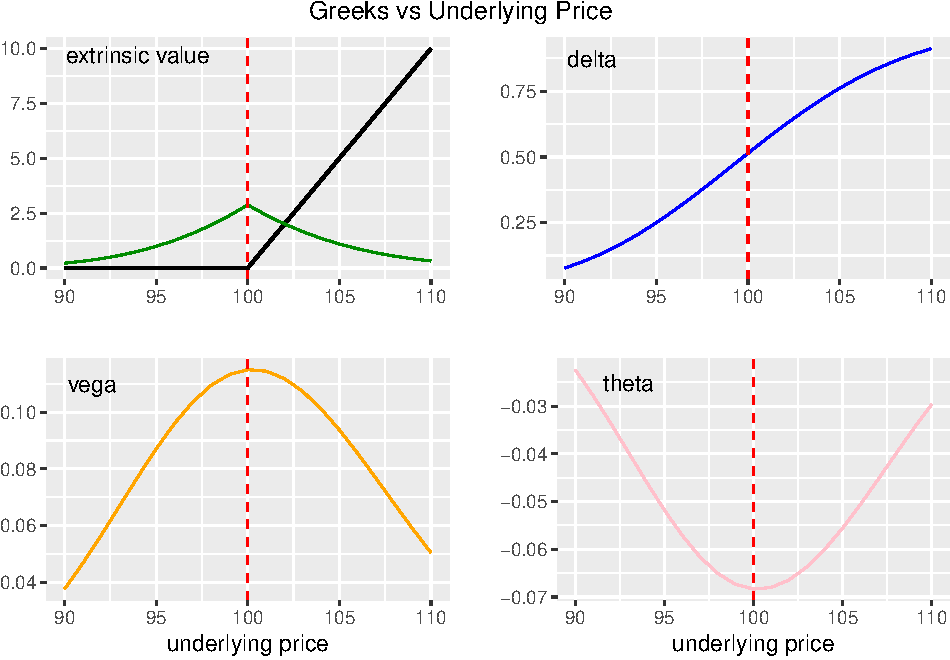
\includegraphics[width=1\linewidth]{rmarkdown_files/figure-latex/greeks_by_moniness-1}

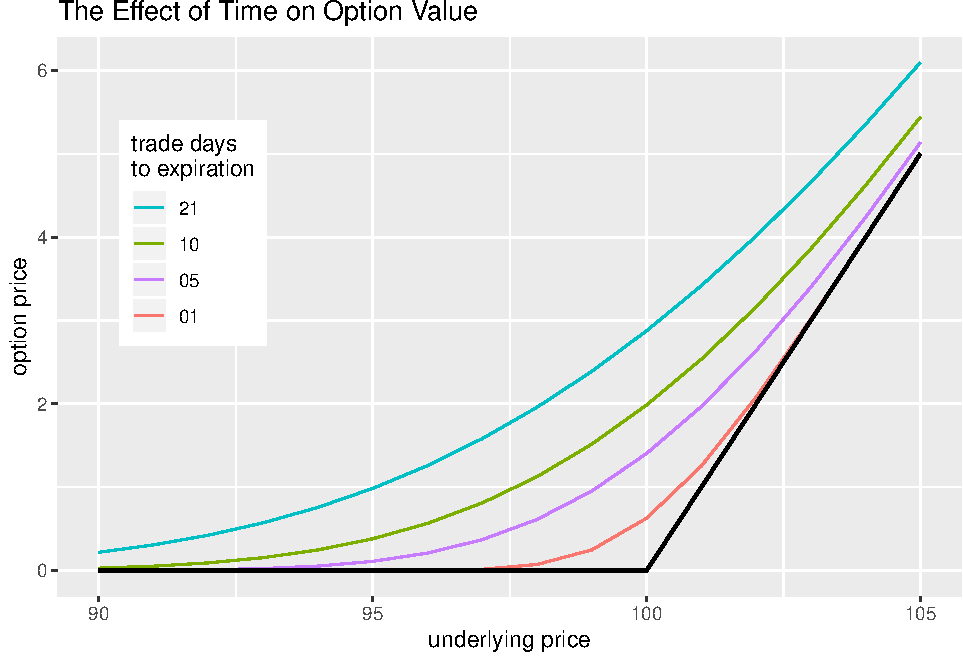
\includegraphics[width=1\linewidth]{rmarkdown_files/figure-latex/option_time_value-1}

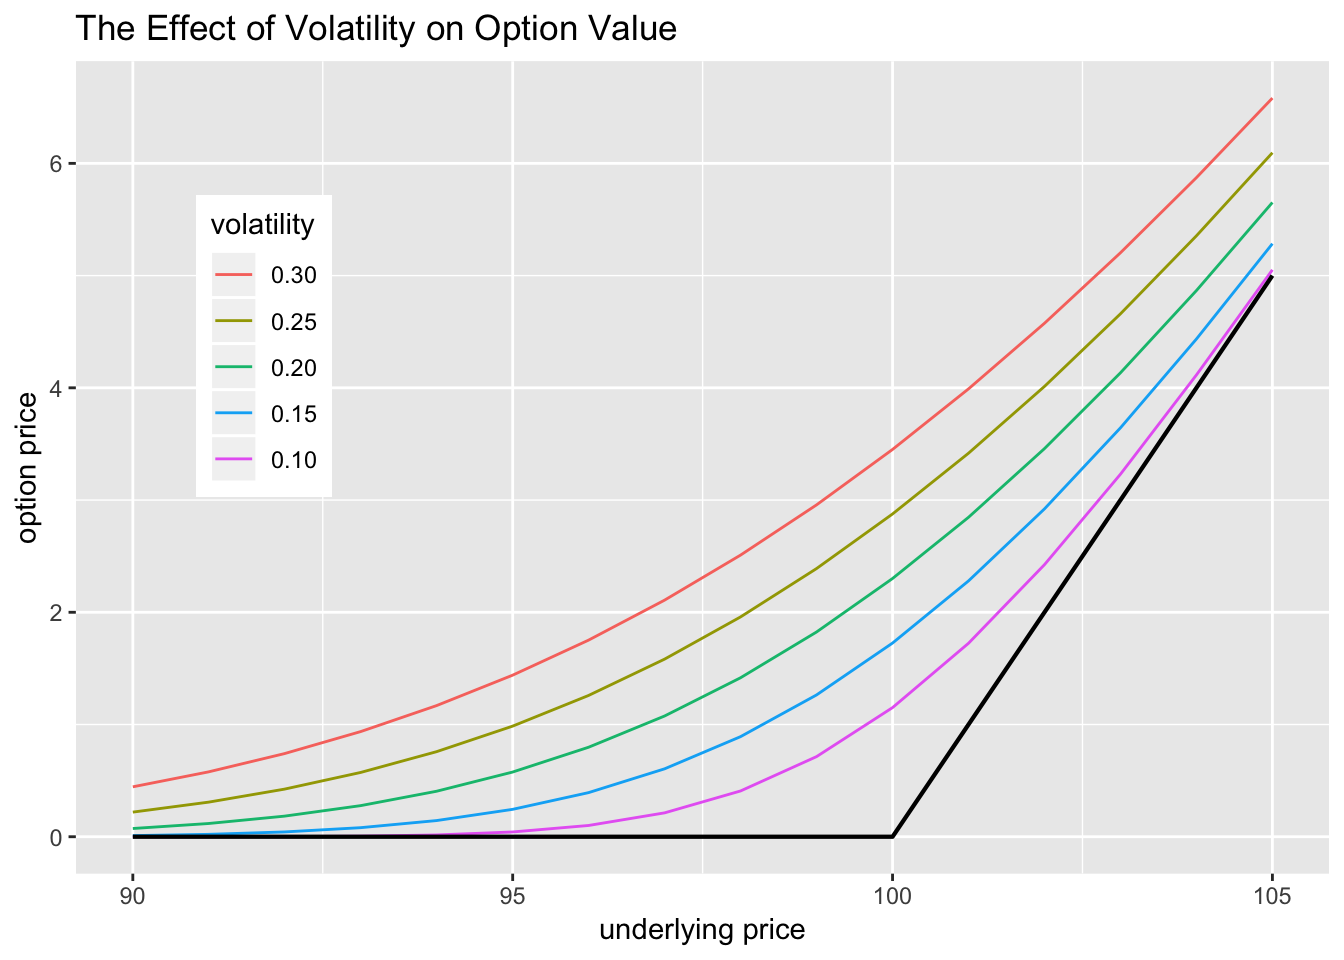
\includegraphics[width=1\linewidth]{rmarkdown_files/figure-latex/option_volatility_value-1}

Here are some observations based on these graphs:

\begin{enumerate}
\def\labelenumi{\arabic{enumi}.}
\item
  Optionality - as evidenced by extrinsic value vega, theta, gamma - is greatest when options are ATM.
\item
  Theta is Negative: an option loses value as it nears expiration.
\item
  Vega is Positive: the more volatile the underlying, the more valuable the option.
\item
  Regarding Delta:

  \begin{itemize}
  \tightlist
  \item
    Approximiately 0.50 when option is ATM.\\
  \item
    Approaches 0.00 as option gets farther out of the money.\\
  \item
    Approaches 1.00 as option goes farther in the money.
  \item
    \emph{VERY roughly} the probability that the option expires ITM.
  \item
    Used to refer to the moniness of an option.
  \end{itemize}
\end{enumerate}

\bibliography{book.bib,packages.bib}

\backmatter
\printindex

\end{document}
